\documentclass[]{report}
\usepackage[T1]{fontenc}
\usepackage[pdftex,bookmarks=true,bookmarksnumbered=true,pdfauthor={Urs Reupke},pdftitle={Anathema User's Guide}]{hyperref}
\usepackage[pdftex]{graphics}
\usepackage{graphicx}
\usepackage{textcomp}
\usepackage{makeidx}
\makeindex

\title{Anathema User Guide\\ Target Program Version: 0.8}
\author{Urs Reupke\\ Original User's Guide written by uteck \\ Anathema created by Sandra Sieroux and Urs Reupke}
\date{}

\begin{document}
\maketitle
\sffamily
\pagenumbering{roman}
\tableofcontents
\pagebreak
\setcounter{page}{1}
\pagenumbering{arabic}

\chapter{Introduction}
\section{About Anathema}
Anathema is a computer toolkit for players of the role playing game of ``Exalted'', published by White Wolf Game Studious of Atlanta, Georgia. It is written in Java and published under the General Public License (GPL).

\section{About this Guide}
This document aims to provide users with an overview of the various functions of Anathema. All modes of usage will be explored and explained in-depth. For those interested in extending the program, instructions will be given.

Each chapter assumes that you have the base knowledge required for using the functions provided. This is no guide to Exalted character design (there are far more proficient people working on that), neither a guide to XML, nor to Java programming. Each of these issues goes far beyond the scope of the guide, but pointers will be given where required.

\section{A History of Exalted Toolkits}
In the beginning, there was White Wolf. The Limited Edition of Exalted featured the demo of a ``soon to come'' character generator for their brand new game. Years passed, Exalted was a huge success, but of the character generator we never heard again.

Next came Jake Baker's Unofficial Exalted Character Generator\footnote{http://sharonandjake.com/jake/freeware/}. It supported a wide variety of character types but was unfortunately not continued into 2003.

That year, however, gave birth to the first public version of EdExalted\footnote{http://www.edexalted.com}. Edward A. Ostrowski provided us with a set of toolkits that is to this date unrivaled in the sheer mass of features. It supports virtually every type of character published for Exalted, comes with a huge database of items and charms and is known to be quite customizable.

The mere existence of EdExalted begs the question: Why Anathema?

\section{Why Anathema?}
\paragraph[Usability.]As great a program EdExalted is when it comes to features, we were quite sad about the user interface. 
Another issue we had were the character sheets generated by the program. While they teem with information, we found them lacking in layout.

\paragraph[Management.]EdExalted is clearly geared towards managing characters, and it does a great job at that. Nevertheless, we realised that there are other issues one faces over the course of a campaign, and we longed for a program to support us with these.

\paragraph[Finally: Curiosity.] Exploring the challenges of modelling a complex set of rules, we wished to see for ourselves what was possible and what was not.
\chapter{Setup}\label{chap:Setup}
This chapter describes all the steps necessary to download, install and configure Anathema. Don't worry - it is not as complicated as it sounds. A standard issue PC and some basic computer skills are all that is required.

\section{System requirements}
While Anathema does not demand anything special in terms of hardware, there is some software that is required to run the program or at least necessary to make the most out of it.

First of all, Java. Anathema is written in the Java programming language and thus needs a working installation of the Java Runtime Environment to run. The minimum Java version required is version 5.0.

If you are already using Java, you can find out what version you are running by opening a console window and typing \texttt{java --version} followed by the \textsc{Enter} key. The resulting output should look something like this:
\medskip
\newline
\small
\texttt{java version "1.5.0\_06"
\newline
Java(TM) 2 Runtime Environment, Standard Edition (build 1.5.0\_06-b05)
\newline
Java HotSpot(TM) Client VM (build 1.5.0\_06-b05, mixed mode)}
\medskip
\newline
\normalsize
The version in this case, repeated in each line, is ``1.5.0\_06''. The relevant digit in our case is the second one: If it is 5 or greater, you're fine.

If it reads lower than 5 or if you do not yet have a copy of the Java Runtime Environment installed, point your web browser to the Java website\footnote{http://java.com/en/download/manual.jsp}, where you can always download the latest version for free.
\medskip
\newline
In addition to Java, you might want a copy of Adobe Reader to view the documents produced. You can get it free of charge from Adobe\footnote{http://www.adobe.com/products/acrobat/readstep2.html}. Of course, any other program capable of displaying PDF files will suffice.

Finally, for greater enjoyment of the music library features, you will need an audio player capable of handling M3U-Playlists ( such as Winamp or XMMS).
\medskip
\newline
Now, with all of that behind us, let's get to the program itself.

\section{Which file to download?}
To download the latest version of Anathema, direct your browser to the Anathema project page\footnote{http://sf.net/projects/anathema} and look for the list of ``Latest File Releases''. Said list contains an entry for package \textsc{anathema}. Click that word, and a screen with a list of all versions released will open.

Note that releases come in two types, \emph{regular releases}, indicated by some Exalted-related name, and \emph{patches}, clearly designated by the word ``patch'' somewhere in the package name.
Regular releases are feature hefty, bringing new functionality and changes. Patches, on the other hand, fix what is broken in a prior release. 
Going from top to bottom, select the first version not labelled as a patch.

Mission accomplished? Great.

Know now that within each package are at least two flavours of Anathema: A \emph{raw} .zip archhive suitable for any operating system and a \emph{Mac OS X} .dmg file. These archive contain everything you need to run Anathema, that is the program itself and a flock of supportive files. 

Occasionally, there might be a third kind of archive, designated \emph{upgrade}. Don't worry about them now, we'll cover them in detail below.

To continue, simply choose the most appropriate package for your operating system, and your download will start. While it is running, you could read on to familiarize yourself with the steps ahead or maybe have a look at our web site to learn about current proceedings.
\medskip

Once the download is finished, you are ready to proceed with the installation.

\subsection{Upgrades and Patches}
If this is your first experience with Anathema, please continue your installation and come back here later to upgrade.

Still there? Alright. So either we screwed up ($\rightarrow$ Patch) or there is cool new stuff to behold ($\rightarrow$ Upgrade). No matter what, your Anathema is outdated, and you want to change it. Here's how.

If there is a more recent version than the one on your system, but we didn't provide an upgrade archive, you will need to go through the installation procedure again. You can safely install the new files over the old installation, just make sure everything is properly overwritten.

If there is an upgrade, download it and extract the files into the old installation directory, overwriting existing files. \emph{Et voil\`a}, you are up to date again.

Upgrade archives are functionally identical to the \emph{raw} version, but are intended for those who already have a running copy of Anathema installed. Lacking the supporting files, they are meant as a way to update the previous version (which also might have been attained by means of upgrade) to the current one. They do not necessarily function with \emph{any} prior version. Not every package contains an upgrade.

Finally, if the new release is a patch, do as you would with an upgrade.As with upgrades, patch archives are not sufficient to run Anathema if it is not already installed and are clearly designated for use with a specific release.

No matter which of the three options it is, your saved files as well as previously made setting stay intact.

\section{Installation}
This step is really simple. Just unzip all the files within to an empty directory, using your favorite archive manager. Make sure that all relative path names are kept, lest Anathema misses some files.

Unless you are using Mac OS X, there is no automated installation mechanism. You will have to make your way to the directory manually, there to launch Anathema. 
\medskip

Let's continue the exploration by starting the program.

\section{Launching Anathema }
There are several ways of starting the program, depending on your operating system.

On most systems you can launch Anathema by opening a console window, changing to the Anathema directory and typing \texttt{java --jar anathema.jar}, followed by a stroke of \textsc{Enter}.
Windows users may opt to use the executable file anathema.exe that comes with the archive or type \texttt{javaw --jar anathema.jar} instead, but this will swallow any error reports that might come up during launch. Also, a freshly installed Java is configured to launch .jar files when they are double clicked in Windows.

A shell script, anathema.sh, is provided for Linux systems. Linux users should make sure that either read-- and write--access are granted on the Anathema directory or that a proper directory is specified at startup. See ``Command Line Options'' below for details.
  
\subsection{Command Line Options}
To submit any optional command line parameter to the launcher, you can put \linebreak
\texttt{-D\emph{[Name\_of\_Option]}} between \texttt{java} and the final argument \texttt{-jar anathema.jar}. Currently, this is only used to supply a custom repository directory.

\begin{description}
\item[repository] - Specifies the directory to use for storage and retrieval. If the directory given does not exist, it will be created if necessary read/write--permissions are granted. If the parameter is omitted, a subdirectory ``Repository'' in the main Anathema folder is assumed to be the repository directory.

	Example:\newline
	\texttt{java -Drepository="C:$\backslash$AnathemaRepository" -jar anathema.jar} will instruct Anathema to store and retrieve data from the directory 
	\linebreak``C:$\backslash$AnathemaRepository''.
	
For future launches, a more permanent way of setting the repository directory is provided. We'll address that in a minute.
\end{description}

\begin{figure}[htb]
	\centering
		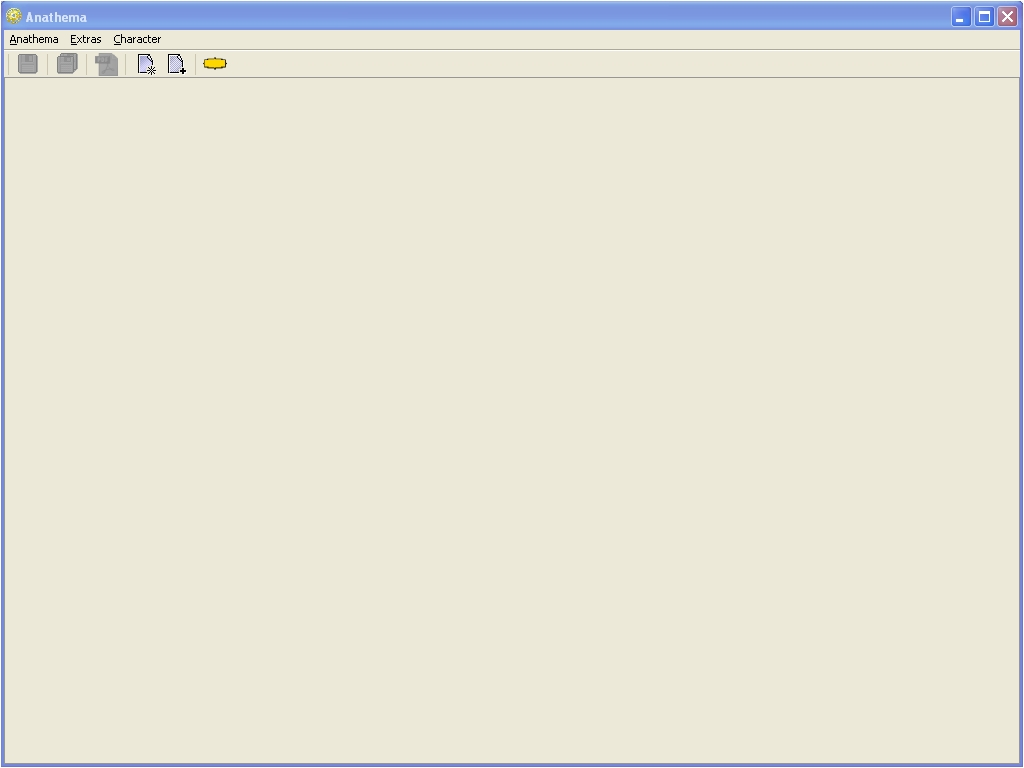
\includegraphics[width=1.00\textwidth]{Images/MainWindow.jpg}
	\caption{The Main Window, Windows Look \& Feel}
	\label{fig:MainWindow}
\end{figure}

\begin{figure}[htb]
	\centering
		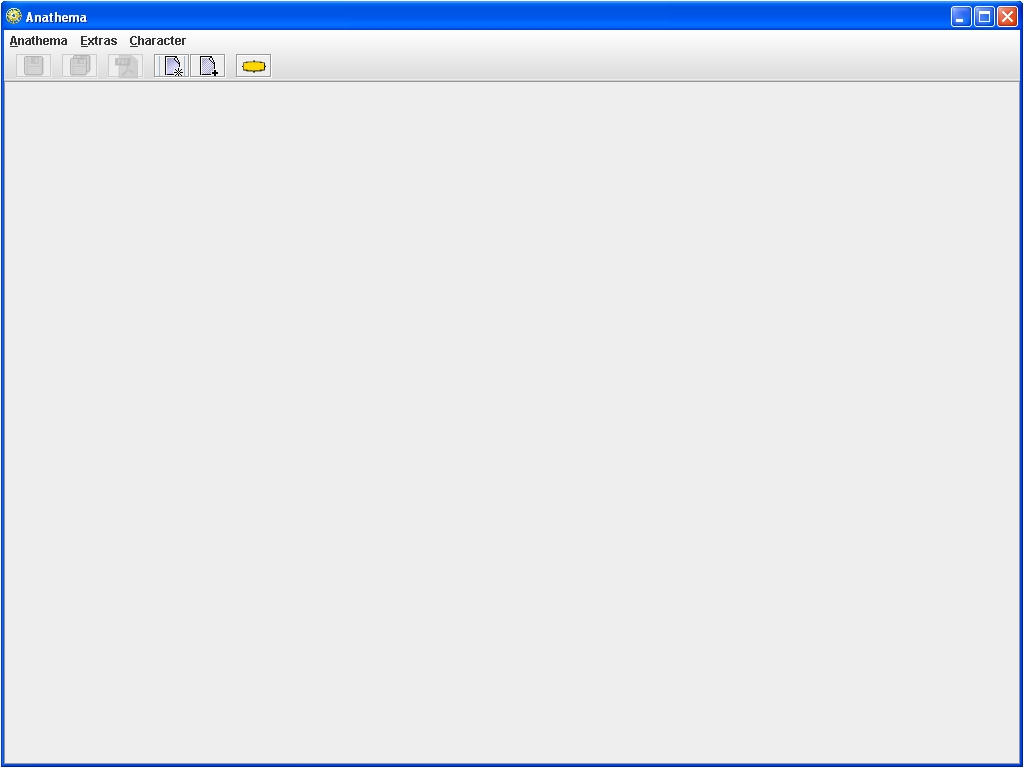
\includegraphics[width=1.00\textwidth]{Images/MainWindowMetal.jpg}
	\caption{The Main Window, Metal Look \& Feel}
	\label{fig:MainWindowMetal}
\end{figure}

\subsection{Done!}
Regardless of the option you chose, Anathema will now load. After a moment's waiting, the splash screen should appear, shortly after to be replaced by the main window. The window on screen should now look similiar to figure \ref{fig:MainWindow} (Windows) or \ref{fig:MainWindowMetal} (everything else).

\textbf{Congratulations!} Your installation of Anathema is now ready to use. Go ahead, fool around! Enter all your favourite characters! Create a new one while you're at it!
\medskip
\newline
Once you're a tad more familiar with the program, come back here and learn about the various settings in the following section.

\section{Setting your Preferences}\label{sec:Preferences}
Tucked away in the menu \emph{Extras} is an entry called \emph{Preferences}. Clicking there unveils a dialog with - who would have thought - various options for Anathema's basic system. The options are stored on a per-user basis, so every account on your system can have it's own settings. Let's have a closer look:
\begin{description}
	\item[Use Metal Look \& Feel] - Available on Windows systems only. Checking the box forces Anathema to use the ``Metal Ocean'' controls instead of the more Windows-like ones used by default. Confer figures \ref{fig:MainWindow} and \ref{fig:MainWindowMetal} for a basic impression.
	\item[Launch maximized] - The Anathema window is maximized at launch. Useful on resolutions of 1024x768, where part of the window might be hidden by operating system controls at the screen's top and bottom.
	\item[Display document after print] - Controls whether PDF documents are opened in your system's default PDF viewer once printing is done.
	\item[Languange] - Selects the language to run the program in. Currently, English and Spanish are available.
	\item[Show tooltips for (seconds)] - This setting, while global, is mainly intended to control the time until displayed Charm details vanish. 
	\item[Repository directory] - The aforementioned option to permanently set the infamous repository directory. Enter a directory or click the browse button for a graphical selection interface. If the directory does not exist, no changes are made to the setting.
\end{description}
	
When everything is set, click \emph{OK} to commit your changes. A dialog will kindly inform you that you need to restart Anathema to see the effects of any changes. You can do so now or at any later point in time. If you clicked \emph{Cancel} instead, the preferences dialog will vanished and all changes are undone.
\medskip
\newline
This concludes the tour of the Anathema setup.

I hope you enjoy the program and stay with us to experience plenty of new versions and features ahead.
\medskip
\newline
Thank you for using Anathema.


\chapter{Management}
This chapter describes those features of Anathema dealing with the bookkeeping aspects of Exalted. All you need is basic familiarity with your computer and the Exalted rules. Copies of the books might come in handy at times, but should not be necessary for understanding.

\section{Basics}
In the following section, you will learn about the basics of item management in Anathema. Items in this case means anything you can create anew and save to disk, later to load it again. Below, you will find explanations of item creation, saving, loading and printing.

\subsection{Item creation}
No matter the type, all items are created by opening the ``Anathema'' menu and pointing towards ``New'', afterwards selecting the item type in question. Depending on the item type chosen, there might be further submenus or dialogs to configure the newly created item.

\subsection{Saving}
When you need to pause editing an item or are truly and utterly done with it, you will want to save your progress. To do so, go the ``Anathema'' menu once more and click the ``Save'' entry. The item will be stored in the repository with a filename depending on both the item type and the name you have given to it. 

Please refer to section \ref{sec:Preferences} for details on customizing the repository directory.

\subsection{Printing}
'Printing' in Anathema is used to output your items to the PDF format.
Select ``Print'' from the ``Anathema'' menu, and a small popup dialog will open, asking you to select the type of report to print the current item in. The options available will, of course, depend on the item type and be explained there.
After choosing the report type, all that is required is a filename to print. 

By default, files will be saved within the Anathema directory with a filename depending on the item name.

\subsection{Loading}
To load an item, simply select ``Load'' from the ``Anathema'' menu. Select the item type to load from the submenu, and a dialog will open, presenting you the previously stored items of the selected type. Select the one you require, and you are done.

\subsection{Recurring Controls}
Some controls are shared by different items. They are collectively explained here for reference.

\subsubsection*{Trait Controls}
Throughout the screens representing a character, you will find rows of dots, either transparent or rendered in a color specific to the character type. These rows, hereafter referred to as ``trait controls'' are used to set your characters various traits.

To use them, either click on the number of dots you wish the trait to have. You can set a value to zero, if allowed, by clicking in the firth third of the first dot. As an alternative, you can click and hold the mouse button. A grey rectangle will appear. Dragging the mouse changes the width of this rectangle, instantly selecting the dots covered.

Trait controls will not allow you to select illegal values for a trait, so if a click yields no reponse or the dots covered by the rectangle are not selected, the values are most probably not allowed by the rules.

\subsubsection*{Formatted Text}
Both notes and series management contain fields in formatted text can be entered. Font options include \textbf{bold}, \textit{italics} or unterlined, to be selected by the controls on the right.

The well established keyboard shortcuts for text formatting, cut and paste operations as well as navigation and selection are also available.

\section{Character Description}\label{sec:CharacterDescription}

\section{Character}
Character items support you in creating and maintaining your character. Among it's features are automatic calculation for point expenditures and generation of character sheets. 

Players use character management to plan and plot their character's advance, while for storytellers it provides the means to be informed of the capabilities of player characters as well as non-player characters.

\subsubsection*{Supported character types}
Anathema supports both Solar and Abyssal Exalted, the Dragon-Blooded as well as Mortals. For most character types, there are various character templates to chose from.

\subsection{Creating a new character}
Together, we will walk through the creation of a new character, from initial creation up to spending the first experience points. Afterwards, everything is up to you.

To create a new character, click Anathema->New->Statted Character. A dialog will open. In there, chose the type of character to create and the ruleset (Core Rules or Power Combat) to use for this character. Both of these settings can't be changed afterwards, so choose wisely.
For purposes of this guide, a ``Loyal Abyssal'' seems like a good choice, since they have some options others are lacking. Confirm the choices made by clicking ``OK''.

After a moment's notice, a item will open.
Three separate areas can be distinguished: The tab area on the upper left, granting access to the different aspects of a character, the overview on the lower left, at all times displaying information about points spent, and the main view, in which the options pertaining to the tab selected are shown.

Right now, we are on the ``Description'' panel, with fields identical to the ``Character Description'' item outlined above (\ref{sec:CharacterDescription}).

Adjusting Values
Throughout Character Creation, you will notice sets of light grey dots - these are to adjust your characters trait values. To select the number of dots assigned to a certain trait, just click on the dots and they will be filled in - alternatively click and keep the mousebutton pressed to be able to drag the value until it's set to the amount you want it to be.
If you want to remove dots, click on the previous dot to remove the next. To remove the first dot, click just before it or in the first third of the dot - again, dragging the selection and releasing the mouse after the value is adjusted will make things easier.
Caste \& Favored Abilities
On the abilities tab, you will note a button in front of each ability. Clicking this button will add it to your Favored Abilities, marked by a highlight.
Caste Abilities are marked with the caste mark.
Magic
The Magic section allows you to choose Charms, spells, and create combos, each on a separate page. Except for some Martial Arts, only Solar Charms can be currently selected. Use the drop list to choose the Group (Ability the Charm is in on and the complete cascade for it will appear. Select Charms by clicking on them and they should turn yellow, indicating a learned charm.This cascade works the same as the separate Cascade function described earlier.
If a Charm is grayed out that means the character has not yet met all prerequisites.
Spells can be learned by selecting them from in the left listbox and clicking the green arrow to the right. To unlearn a spell, select it, then click the red "X".
Combo creation is similar to spell selection: Simply select one charm at a time and click the green arrows to add it to the current combo, afterwards enter a name and short description of the combo, then click the green + to finalize the combo. The center button can be used to clear the combo currently edited and start over.
Overview
The Overview on the left will keep track of the choices you made, automatically adjusting if you change things. Colors and font show the state of the item displayed:
Purple indicates that you still need to spend points, while black means that everything allotted is spend. Items on which you spend bonus points (which are calculated automatically) are shown bold. If the Bonus Points counter at the bottom becomes red, this means that you have overextended your amount allowed bonus points.
Number in parentheses indicated that the characters absolute maximum has somehow been raised above the maximum (eg. a larger than usual Essence Pool), while a second number delimited by a "+" notifies you of additional Points to spend.
For example, if I put 8 dots in Physical, and 6 in Mental, then remove 2 dots from Physical, the Promary will list 6/8 meaning only 6 points of 8 have been spent. If I then add them to Mental, it becomes the Primary and is then listed as 8/8. If I spend a 9th dot the Primary line becomes Bold, and the Bonus Points, at the bottom of the left side, is incremented to show that 4 points has been spent to increase the Attribute.

\subsection{Experience}
Once character creation is finished, the character can be further advanced within the program, but first, you have to convert it to 'experienced mode' by clicking the equinymous entry in the 'Character' menu.
After clicking, you'll notice a change in the overview window - it now shows your current XP breakdown - as well as a new tab for the character - within, you'll find a table in which to enter the experience awards for your character.To do so, just add an entry by clicking the '+' and adjust the number. You can also add a comment for later reference.
From now on, your character's stats cannot be lowered below the values you've set during creation, and any adjustments you make will be paid for with experience, their cost being calculated automatically.

\section{Series Management}
Series management is currently limited to plot management.

Usage is straightforward: To the left of the screen, the series plot tree is displayed. 

Use the right-click context-menu or the buttons provided at the screen's bottom to add Stories, Episodes and Scenes to the plot outline. Afterwards select an entry in the outline to enter a title and an description for the proceedings within, either planned or already passed.

An item can be moved among it's peers via the up/down controls next to the add/remove buttons. Drag-and-dropping allows to attach child items to different parents.

\section{Notes}
Notes are the most basic type of item known to Anathema. They consist of nothing more than a title and a formatted text field, allowing you to keep track of things fitting nowhere else or preparing simple texts for game sessions.

Printing is currently not available for notes.

\section{Music Database}
One of the more unusual features of Anathema's is the Music Database. This module, which could as well be seen as a stand-alone program, is used to prepare a database of mp3-files for use at the gaming table. Tracks can be categorized by three different types of keywords, stored in playlists and sought for by various parameters. This section explains the options the Music Database offers.

\subsection{Libraries}
\subsection{Selections}
\subsubsection*{Current Selections}
\subsubsection*{Stored Selections}
\subsection{Track Details}
\subsubsection{Categories}
\subsection{Search}

\chapter{Extras}
The Extras menu contains features that do not deal with items created for your campaign. The Charm Cascades module provides convenient access to the entire charm database, while the preferences dialog gives you some degree of freedom on the program's basic behaviour.

\section{Charm Cascades}
The Charm Cascades module allows you to browse the entire Anathema Charm database without being limited to those charms available to your character. Currently, Charms for the supported character types as well as Sidereal Exalted are included.

\subsection{Using charm cascades}
To view the Charm Cascades, either press the yellow button in the toolbar (it vaguely resembles a Solar Charm icon) or select "Show Charm Cascades" from the ``Extras'' menu. 

\begin{figure}[htb]
	\centering
		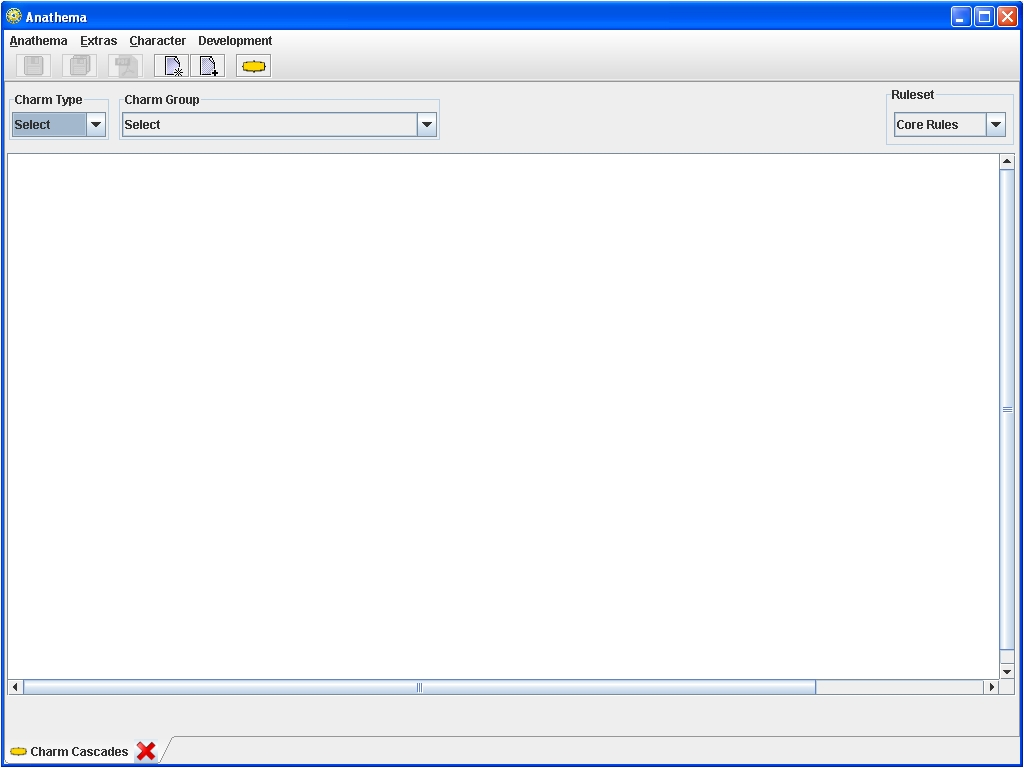
\includegraphics[width=1.00\textwidth]{Images/CharmCascadesEmpty.jpg}
	\caption{Charm Cascades view, immaculate}
	\label{fig:CharmCascadesEmpty}
\end{figure}

A new Tab will open, as depicted in figure \ref{fig:CharmCascadesEmpty}. Within, you will see three drop-down lists at the top and a vast, empty area below. Use the first drop-down, ``Charm Type``, to switch between the various character types and Martial Arts. Once done, the second drop-down box will be filled with the various charm groups for the type selected.

At a moments notice, the background of the canvas will change to the selected types color, shortly after, the charm tree for the selected group will be displayed. The graphics are closely modeled after the examples given in the Exalted rulebooks, so you should have no trouble finding your way around.

\begin{figure}[htb]
	\centering
		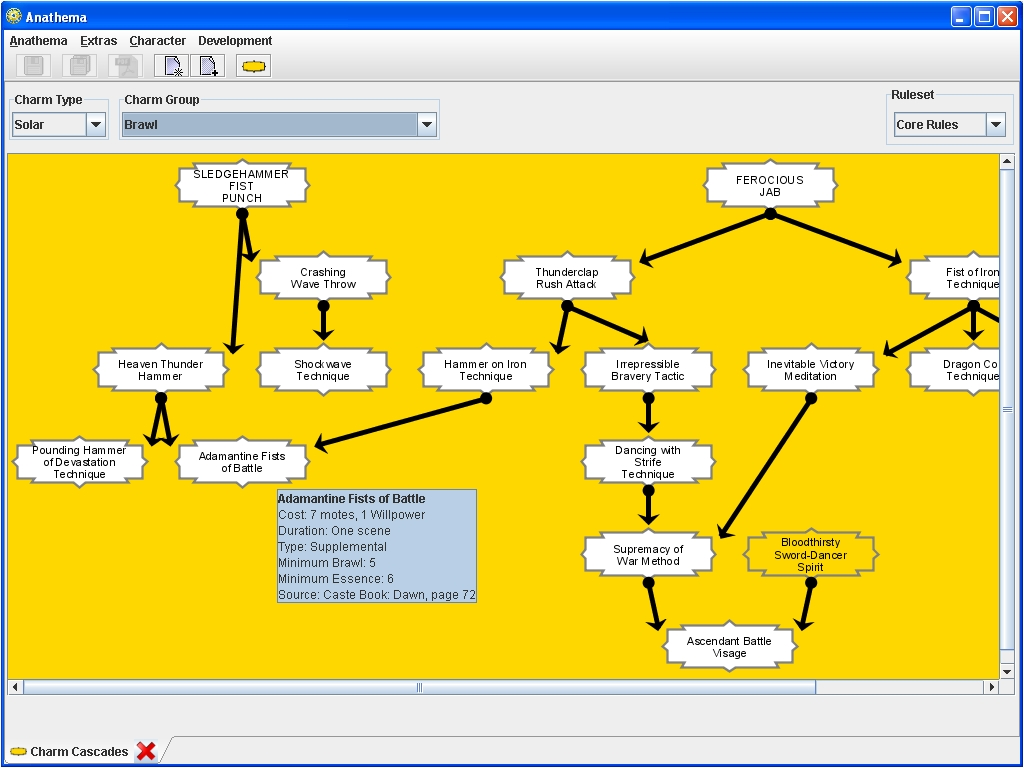
\includegraphics[width=1.00\textwidth]{Images/CharmCascadesTooltip.jpg}
	\caption{Charm Cascades view, tooltip showing}
	\label{fig:CharmCascadesTooltip}
\end{figure}

The only difference between Anathema's rendition and those familiar depictions is the way Charms from groups different than the current one are displayed: To clearly mark these 'external' charms, they are rendered not in white, but with a transparent background. An example of this can be seen at the lower right of figure \ref{fig:CharmCascadesTooltip}.

You can hover the mouse cursor over any of the charm symbols to trigger a tooltip with closer information on that charm: The entire block of statistics as well as a source are given. Refer to figure \ref{fig:CharmCascadesTooltip} for a rough impression. 'External' charms won't display any information.

The exact content displayed in the tooltip depends on the ruleset chosen, which is done by the third box above. Current selections include the Core Rules and the changes wrought by the introduction of Power Combat.

\section{Preferences}
The preferences dialog allows you to customize various aspects of Anathema. Please see section \ref{sec:Preferences} for a detailed explanation of the various options.
\chapter{Customizing}
\chapter{Future development}
\section{Planned Features}
\section{Feature Requests}

\begin{appendix}
\chapter{Development Environment}

\section{CVS Projects}
\texttt{include CurrentProjects.txt}

\section{An Introduction to Modules}
\texttt{include ExplanationOfModules.txt}

\section{Software}
%Was f�r Software wir wof�r benutzen
%Eclipse with Ant, JUnit and Continuous Testing, JDemo
%GIMP
%LaTeX, MikTex, TeXnicCenter

\chapter{Format explanations}
This appendix contains the XML schemas defining the various formats defined for use with Anathema. 

For a short explanation of the M3U playlist format, please read the relevant article at AssistantTools.com\footnote{http://www.assistanttools.com/articles/m3u_playlist_format.shtml}.
\section{Note Files}
\section{Character Files}
\section{Series Files}
\section{Charm Files}
\printindex
\bibliography{Anathema}
\bibliographystyle{unsrt}
\end{appendix}
\end{document}